%&latex

\documentclass[12pt,a4paper]{article}

\usepackage[T1]{fontenc}
\usepackage{amsfonts}
\usepackage{amsmath}
\usepackage{amsthm}
\usepackage{amssymb}
\usepackage[all]{xy}
\usepackage[nice]{nicefrac}
\usepackage{color}
\usepackage{graphicx}

\hbadness=10000
\vbadness=10000

\setlength{\oddsidemargin}{.25in}
\setlength{\evensidemargin}{.25in}
\setlength{\textwidth}{6in}
\setlength{\topmargin}{-0.4in}
\setlength{\textheight}{8.5in}

\newcommand{\symdiff}{\bigtriangleup}
\newcommand{\set}[1]{{\left\{#1 \right\}}}
\newcommand{\zo}{ \left\{0,1\right\} }
\newcommand{\pmone}{ \left\{ \pm 1\right\} }
\newcommand{\0}{{\bf 0}}
\newcommand{\RM}{\mathcal{RM}}
\newcommand{\D}{\Delta}
\newcommand{\A}{{\mathcal{A}}}
\newcommand{\B}{{\mathcal{B}}}
\newcommand{\T}{{\mathcal{T}}}
\newcommand{\F}{{\mathcal{F}}}
\newcommand{\G}{{\mathcal{G}}}
\newcommand{\U}{{\mathcal{U}}}
\newcommand{\RR}{{\mathcal{R}}}
\newcommand{\FF}{{\mathbb F}}
\newcommand{\N}{{\mathbb N}}
\newcommand{\Z}{{\mathbb Z}}
\newcommand{\R}{{\mathbb R}}
\newcommand{\C}{{\mathbb C}}
\newcommand{\Q}{{\mathbb Q}}
\renewcommand{\S}{{\mathbb S}}
\newcommand{\eqdef}{{\stackrel{\rm def}{=}}}
\newcommand{\ip}[1]{{\left\langle #1 \right\rangle}}
\renewcommand{\span}{{\rm span}}
\newcommand{\poly}{{\rm poly}}
\newcommand{\ftilde}{\widetilde{f}}
\newcommand{\gtilde}{\widetilde{g}}
\newcommand{\fhat}{\hat{f}}
\newcommand{\hhat}{\hat{h}}
\newcommand{\ghat}{\hat{g}}
\newcommand{\otn}{{\otimes n}}
\newcommand{\tnpar}[2]{{{\otimes}^{#1}{#2}}}
\newcommand{\tn}{{\overset{t}{\otimes}n}}
\newcommand{\Tn}{T^{\otimes n}}
\newcommand{\Sn}{S^{\otimes n}}
\newcommand{\Tntilde}{\tilde T^{\otimes n}}
\renewcommand{\a}{\alpha}
\renewcommand{\b}{\beta}
\renewcommand{\d}{\delta}
\newcommand{\la}{\langle}
\newcommand{\ra}{\rangle}
\newcommand{\four}{\{0,1,2,3\}}
\newcommand{\ol}{\overline}
\newcommand{\chop}{\mathrm{chop}}
\newcommand{\eps}{\epsilon}
\newcommand{\seq}{\subseteq}
\newcommand{\suq}{\supseteq}
\newcommand{\norm}[1]{\left\| #1 \right\|}
\newcommand{\E}{{\mathbb E}}
\newcommand{\Var}{{\rm Var}}
\def\half{\frac{1}{2}}
\def\nicehalf{\nicefrac{1}{2}}
\def\quarter{\frac{1}{4}}
\def\nicequarter{\nicefrac{1}{4}}
\newcommand\col[2]{\textsc{Approx}\-\textsc{Coloring}({#1},{#2})}
\newcommand{\One}{{\bf 1}}
\newcommand{\Inf}[1]{{\rm Inf}_{#1}}
\newcommand{\XInf}[1]{{\rm XInf}_{#1}}
\renewcommand{\bar}{\overline}
\newcommand{\supp}{{\sf supp}}

\newtheorem{theorem}{Theorem}[section]
\newtheorem{corollary}[theorem]{Corollary}
\newtheorem{proposition}[theorem]{Proposition}
\newtheorem{definition}[theorem]{Definition}
\newtheorem{lemma}[theorem]{Lemma}
\newtheorem{claim}[theorem]{Claim}
\newtheorem{observation}[theorem]{Observation}
\newtheorem{notation}[theorem]{Notation}
\newtheorem{fact}[theorem]{Fact}
\newtheorem{assumption}[theorem]{Assumption}
\newtheorem{conjecture}[theorem]{Conjecture}
\newtheorem{goal}[theorem]{Goal}
\newtheorem{question}[theorem]{Question}


\newenvironment{quotetheorem}[1]{\par\noindent{\bf #1}\hspace*{1em}}{\bigskip\par}

%\newenvironment{proof}{\noindent{\bf Proof}\hspace*{1em}}{\qed\bigskip}
\newenvironment{proof-sketch}{\noindent{\bf Sketch of Proof}\hspace*{1em}}{\qed\bigskip}
\newenvironment{proof-idea}{\noindent{\bf Proof Idea}\hspace*{1em}}{\qed\bigskip}
\newenvironment{proof-of-lemma}[1]{\noindent{\bf Proof of Lemma #1}\hspace*{1em}}{\qed\bigskip}
\newenvironment{proof-of-thm}[1]{\noindent{\bf Proof of Theorem #1}\hspace*{1em}}{\qed\bigskip}
\newenvironment{proof-attempt}{\noindent{\bf Proof Attempt}\hspace*{1em}}{\qed\bigskip}
\newenvironment{proofof}[1]{\noindent{\bf Proof of #1:}\hspace*{1em}}{\qed\bigskip}
\newenvironment{remark}{\noindent{\bf Remark}\hspace*{1em}}{\bigskip}
\newenvironment{remarks}{\noindent{\bf Remarks}\hspace*{1em}}{\bigskip}

\newenvironment{reduction}{\noindent{\bf \large Reduction}\hspace*{1em}}{\bigskip}
\newenvironment{completeness}{\noindent{\bf Completeness}\hspace*{1em}}{\qed\\}
\newenvironment{soundness}{\noindent{\bf Soundness}\hspace*{1em}}{\qed\\}

\newcommand{\itemlist}[1]{\begin{itemize}#1\end{itemize}}
\newcommand{\enumlist}[1]{\begin{enumerate}#1\end{enumerate}}
\newcommand{\desclist}[1]{\begin{description}#1\end{description}}
\newcommand{\eqnar}[1]{\begin{eqnarray*}#1\end{eqnarray*}}


\begin{document}

\title{\bf Greedy Random Walk}
\author{Tal Orenshtein\thanks{\scriptsize{Department of Mathematics, Weizmann Institute of Science, Rehovot, Israel. talo@weizmann.ac.il, http://www.orenshtein.com}} \and Igor Shinkar\thanks{\scriptsize{Department of Computer Science and Applied Mathematics, Weizmann Institute of Science, Rehovot, Israel. igor.shinkar@weizmann.ac.il}}}

\date{}
\maketitle

\abstract
A greedy random walk on a graph is the following discrete time self interacting random process.
Each vertex maintains the set of adjacent edges touching it yet to be crossed.
At each step, if the walk is in some vertex, it picks an edge uniformly at random among the adjacent edges of that vertex yet to be traversed. If all its adjacent edges have been crossed, then an adjacent edge is picked uniformly at random. After picking an edge the walker jump along it to a neighboring vertex. Several results are presented
regarding edge cover-time and transience.

%%%%%%%%%%%%%%%%%%%%%%%%%%%%%%%%%%%%%%%%%%%%%%%%%%%%%%%%%%%%%%%%%%%%%%%%%%%%%%%%%%%%%%%%%%
\section{Introduction}\label{sec:intro}
%%%%%%%%%%%%%%%%%%%%%%%%%%%%%%%%%%%%%%%%%%%%%%%%%%%%%%%%%%%%%%%%%%%%%%%%%%%%%%%%%%%%%%%%%%

{\it Greedy random walk} (GRW) on a graph $G=(V,E)$ is a discrete time random process, with a transition law defined as follows.
Each vertex $v \in V$ maintains the set of adjacent edges touching it, that the walker hasn't crossed yet.
At each step from vertex $v \in V$, the walker picks uniformly at random an unvisited edge,
and if all the adjacent edges have been visited, an adjacent edge is picked uniformly at random.
Then the walker jumps along the picked edge to a neighboring vertex.
\medskip

Formally, a greedy random walk is a sequence $X_0,X_1,X_2, \dots$ of random variables defined on $V$, with the following transition probabilities.
For each time $t \geq 0$ define
\[
    H_t = \set{\set{X_{s},X_{s+1}} \in E : 0 \leq s < t}
\]
to be the set of all the edges traversed by the walk up to time $t$.
For every vertex $v \in V$ and time $t \geq 0$ define
\[
    J_t(v) = \set{e \in E : v \in e \text{ and } e \notin H_t}
\]
to be the set of all the edges touching $v$ that have not been traversed by the walk up to time $t$.
The transition probabilities are given by:
\[
    \Pr[X_{t+1} = w | X_1, \dots, X_t] =
        \begin{cases}
            \frac{1}{|J_t(X_t)|}    &  J_t(X_t) \neq \emptyset \text{ and } \{X_t,w\} \in J_t(X_t) \\
            \frac{1}{|N_{X_t}|}     &  J_t(X_t) = \emptyset \text{ and } w \in N_{X_t} \\
            0                       &  \text{ otherwise }
        \end{cases}
\]
where $N_v$ is the set of neighbors of $v$ in $G$.
\medskip

This variant of self interacting walk is related to bridge burning RW
which is repelling rather than the attracting reinforced RW, rotor
router RW, non-backtracking RW and excited RW, see \cite{Pem07} for background,
(see also \cite{FrSa10}, \cite{ABLS06}, \cite{BW03})

One motivation for the study the GRW is arising from distributed computation in which on each vertex of the graph sits an agent,
each agent knows and can communicates only with his neighbors.
The goal of the agents is as fast as possible to let as many of the agents use some resource,
while using no extra information regarding the graph and the vertices that were already visited.
An agent has only a list of neighbors who communicated with him thus far.
Each time the agent receives the resource, it can move it only to one neighbor.
We will see that  the GRW protocol can preform better than simple random walk (SRW) on some graphs.

The repelling nature of GRW suggests that the range of the walk will
grow at least as fast as that of SRW and that it will mix at least as fast as SRW.
We will study the cover time of finite graphs by the GRW, and
establish faster GRW cover time for a few natural families of graph.
E.g.\ the expected time it takes the GRW to go via all edges
of the complete graph of size $n$ is $\Theta(n^2)$.
Recall that Feige \cite{Feige95lowerbound} showed that the expected cover time of a
graph of size $n$ by a simple random walk is at least $n \log n$,
and recently in \cite{BGM} it was shown that for bounded degree graphs linear cover time is
exponentially unlikely.

For many years probabilists are clueless regarding some
basic conjectures about self interacting random walks. Occasionally
some combinatorial observation, a coupling technique
or other insights allow the analysis of such a process. We will see
below that this is the case for the GRW, thus easily proving that
GRW is transient on $Z^d, d >2$. The current simple proof totally
depends on the degrees of the graph being even and we don't know
how to handle odd degrees at all. This suggests several conjectures.
\medskip


\medskip

The next section is regarding covertime of finite graphs. Then we move to GRW on $\Z^d$.
We end with a list of open problems.






%%%%%%%%%%%%%%%%%%%%%%%%%%%%%%%%%%%%%%%%%%%%%%%%%%%%%%%%%%%%%%%%%%%%%%%%%%%%%%%%%%%%%%%%%%
\section{Edge cover time on finite graphs}\label{sec:edge_cover_time}
%%%%%%%%%%%%%%%%%%%%%%%%%%%%%%%%%%%%%%%%%%%%%%%%%%%%%%%%%%%%%%%%%%%%%%%%%%%%%%%%%%%%%%%%%%

    Let $G=(V,E)$ be a connected undirected finite graph on $n$ vertices.
    We denote by $T^E_G$ the number of steps it takes for the greedy random walk to traverse all edges of $G$. Note that since $G$ is a finite graph, $T^E_G$ is a.s.\ finite.
    Since the restriction on the random walk is with respect to the adjacent edges of the current vertex,
    it seems more natural to ask about the edge cover time, rather than vertex cover time.
    We hope that for many interesting families of graphs, the greedy walk covers the edges asymptotically faster
    than the simple random walk. We are able to show it on several natural families of graphs.
    \medskip

    The basic idea is as following.
    Divide the GRW into two random parts:
    \enumlist{
        \item The greedy parts - all steps that cover the yet uncovered edges.
        \item The simple parts - all steps that traverse all the edges that have already been covered previously,
                                i.e.\ the choice of edges is distributed according to the distribution of the simple random walk.
    }

    Roughly speaking, the GRW typically looks as following: It starts with a greedy part. The greedy part continues until
    reaching at time $s_1$ a vertex $v_1$ whose all edges have already been covered.
    We think in this situation that the walk got stuck.
    This means that the last step before getting stuck, covered the last edge touching $v_1$.
    Since all edges touching $v_1$ have been covered, the walk picks an edge at random among the already covered edges.
    In other words the walk is in a simple part.
    The simple part continues until the simple walk reaches at time $t_1$ a vertex $u_1$ that has an uncovered edge touching it.
    By definition, the next step will belong to a greedy part and will continue until reaching at time $s_2$
    to some vertex $v_2$ whose all edges have already been covered, starting the second simple part.
    The second simple part will end when the walk reaches at time $t_2$ a vertex $u_2$ that has an uncovered edge touching it.
    The walk continues like this until all edges are covered.

    Formally, define inductively for $i \geq 0$
    \eqnar{
        t_0 & = & 0 \\
        s_{i+1} & = & \inf  \set{t > t_i : J_t(X_t)  = \emptyset} \\
        t_{i+1} & = & \inf \set{t > s_{i+1} : J_t(X_t)  \neq \emptyset}
    }
    This gives us a random partition $(t_0 = 0,s_1,t_1,s_2,t_2,\dots,s_k)$
    of the time segment $[0, T^E_G]$.
    Note that $H_{s_k} = E$.
    We say the walk \emph{got stuck} at time $t$ if $t = s_i$ for some $i = 1, \dots, k$.
    It should be clear from the description, that the vertices $X_{s_i}$ must all be distinct,
    as $X_{s_i}$ is exactly the $i$-th time that the walk got stuck and it is impossible to get stuck in the same vertex twice.
    In particular $k \leq n$.

    Note that in any walk the total size of the greedy parts equals exactly to the number of edges $|E|$.
    Thus in order to bound $\E[T^E_G]$, we need to bound the expected size of each simple part $\E[t_i - s_i]$,$i = 1, \dots, k$.

    We say a vertex $v$ at time $t$ is \emph{occupied} if $J_t(v) = \emptyset$,
    i.e.\ all edges adjacent to $v$ are covered by time $t$.
    Define $B_i$ to be
    \[
        B_i = \set{v \in V : J_{s_i}(v) = \emptyset}
    \]
    the set of all occupied vertices by time $s_i$.
    By the definition of $s_i$ and $t_i$ we note that
    $B_i = \set{v \in V : J_{t}(v) = \emptyset}$ for every $t \in [s_i, t_i]$.
    Note that $B_j \seq B_i$ for all $j \leq i$ and $X_{s_j} \notin B_i$ for $j > i$.
    Thus $B_1 \subset B_2 \subset ... \subset B_k = V$, where all the containments are strict.

    Having defined $B_i$, it is easy to see that the length of the time segment $[s_i, t_i]$
    equals exactly the escape time of a simple random walk from $B_i$ when started at $X_{s_i}$.
    That is $t_i - s_i = T(X_{s_i},B_i)$, where
    \[
        T(v,B) = \min\set{t: X_t \notin B | X_0 = v}
    \]
    Since the behavior of the walk in the time segment $[s_i, t_i]$ is a simple random walk,
    we can apply known results regarding SRW to bound the expected escape time.

    We apply this idea to several families of graphs,
    showing that the expected edges cover time of the GRW is asymptotically faster than that of SRW.

%%%%%%%%%%%%%%%%%%%%%%%%%%%%%%%%%%%%%%%%%%%%%%%%%%%%%%%%%%%%%%%%%%%%%%%%%%%%%%%%%%%%%%%%%%
\subsection{Clique}\label{subsec:cluque}
%%%%%%%%%%%%%%%%%%%%%%%%%%%%%%%%%%%%%%%%%%%%%%%%%%%%%%%%%%%%%%%%%%%%%%%%%%%%%%%%%%%%%%%%%%

    Consider $G = K_n$, the complete graph of $n$ vertices.
    A simple observation here is as following:
    For any $i = 1 \dots k$, the expected escape time from $B_i$ is distributed geometrically
    \[
        t_i - s_i \sim G(1 - \frac{|B_i|}{n})
    \]
    Therefore
    \[
        \E[t_i - s_i] = \frac{n}{n - |B_i|}
    \]
    Since $B_i$ form a strict chain, we have a bound of the sum of the expectations.
    \[
        \sum_{i=1}^k \E[t_i - s_i]  = \sum_{i=1}^k \frac{n}{n - |B_i|} \leq \sum_{i=1}^n \frac{n}{n - i}
    \]
    Summing over all $i$'s gives the following result for cliques.
    \begin{proposition}\label{thm:clique}
        Let $G = K_n$. Then the expected edge cover time of GRW on $K_n$ has
        \[
            \E[T^E_{K_n}] \leq |E| + n \log(n) = (1 + o(1))|E|
        \]\qed
    \end{proposition}
    This is an improvement over the $\Omega (n^2 \log(n))$ time of the SRW.

    A remarkable fact recently proved by Omer Angel and Yariv Yaari states that the expected number of unvisited edges
    in the $n$-complete graph until the first time the walk got stuck (i.e.\ up to time $s_1$) is linear in $n$, for $n$ odd \cite{AngelYaari}.

%%%%%%%%%%%%%%%%%%%%%%%%%%%%%%%%%%%%%%%%%%%%%%%%%%%%%%%%%%%%%%%%%%%%%%%%%%%%%%%%%%%%%%%%%%
\subsection{Expanders}\label{subsec:expanders}
%%%%%%%%%%%%%%%%%%%%%%%%%%%%%%%%%%%%%%%%%%%%%%%%%%%%%%%%%%%%%%%%%%%%%%%%%%%%%%%%%%%%%%%%%%

    We apply the same techniques on $(n,d,\lambda)$-expander graphs.
    We are able to show that for $d = \log(n)$, the greedy edge cover time is linear in the number of edges.
    This is faster than a simple random walk, which covers the edges in $\Omega ( |E| \log |E| )$ steps.

    \begin{theorem}\label{thm:spectral_bound}
        Let $G$ be any $(n, d, \lambda)$-graph.
        Then $\E[T^E_G] \leq |E| + O \left( \frac{n \log(n)}{1-\lambda} \right)$.
        In particular for an expander with $d = \log(n)$ the expected greedy edge cover time is linear in the number of edges.
    \end{theorem}

    \begin{proof}
    We upper bound the quantity $t_i - s_i$ using the lemma due to Broder and Karlin.

    \begin{lemma}[\cite{BroderKarlin89} Lemma 3]
        Let $G$ be an $(n,d,\lambda)$-graph and let $B \seq V$ be a set of vertices.
        Consider a random walk $X_0, X_1 \dots$ from some $v \in B$.
        Recall that $T(v,B)$ is the escape time of the walk from $B$ when started from $v$.
        Then
        \[
            \E[T(v,B)] \leq \left( \frac{O( \log(n) ) + \frac{n}{n-|B|}}{1 - \lambda} \right) (1 + o(1))
    \qedhere\]
    \end{lemma}
    Plugging into the lemma, we have
    \[
        \E[t_i - s_i]  \leq  \left( \frac{O( \log(n) ) + \frac{n}{n-|B_i|}}{1 - \lambda} \right) (1 + o(1))
    \]
    Summing over all $i$'s we get
    \[
        \sum_{i=1}^{k} \E[t_i - s_i] \leq \sum_{i=1}^k \left( \frac{O( \log(n) ) + \frac{n}{n-|B_i|}}{1 - \lambda} \right) (1 + o(1))
                \leq O \left(\frac{n \log(n)}{1 - \lambda} \right)
    \]
    which completes the proof. \qed
    \end{proof}

    We do not know if for a bounded degree expander the greedy edge cover time is $o(n \log n)$.

%%%%%%%%%%%%%%%%%%%%%%%%%%%%%%%%%%%%%%%%%%%%%%%%%%%%%%%%%%%%%%%%%%%%%%%%%%%%%%%%%%%%%%%%%%
\subsection{Hypercube $\zo^d$}\label{subsec:zo^d}
%%%%%%%%%%%%%%%%%%%%%%%%%%%%%%%%%%%%%%%%%%%%%%%%%%%%%%%%%%%%%%%%%%%%%%%%%%%%%%%%%%%%%%%%%%

    As a corollary from the previous result we obtain a bound on the $\zo^d$ hypercube.
    The bound is useful (improves over the SRW) only
    when we connect two vertices if the hamming distance between them is $\ell$, for some $\ell \geq 2$ (and not $1$ as usual).
    We do not know whether for the usual hypercube graph $\E[T^E_G]$ is smaller that $O(n \log^2(n))$.

    \begin{proposition}\label{thm:zo^d}.
        Let $G=(V,E)$ be the $d$ dimensional hypercube graph, where $(x,y) \in E$ iff $d(x,y) = \ell$.
        That is $n = |V| = 2^d$ and $|E| = \Theta( {d \choose \ell} \cdot 2^d )$.
        Then $\E[T^E_G] \leq |E| + O ( n \log^2(n) )$.

        The assumption $d(x,y) = \ell$ can be replaced by $d(x,y) \leq \ell$.
    \end{proposition}

    \begin{proof}
        The proof is just by plugging the second eigenvalues associated with $G$, $\lambda = 1 - \Theta_\ell(\log^{-1}(n))$ in Theorem \ref{thm:spectral_bound},
        implying $\E[T^E_G] \leq |E| + O ( n \log^2(n) )$.
    \end{proof}

%%%%%%%%%%%%%%%%%%%%%%%%%%%%%%%%%%%%%%%%%%%%%%%%%%%%%%%%%%%%%%%%%%%%%%%%%%%%%%%%%%%%%%%%%%
\subsection{$d$-trees}\label{subsec:binary_tree}
%%%%%%%%%%%%%%%%%%%%%%%%%%%%%%%%%%%%%%%%%%%%%%%%%%%%%%%%%%%%%%%%%%%%%%%%%%%%%%%%%%%%%%%%%%

    So far we considered graphs with superconstant degree.
    We are also able to upper bound the edge cover time of GRW on trees.

    \begin{theorem}\label{thm:trees}
        Let $G = (V,E)$ be any tree rooted at $r$ such that $\deg(r) \geq 2$.
        For any $v \in V$ denote by $T_v$ the subtree rooted at $v$
        and let $|T_v|$ denote the number of edges in $T_v$.
        Then the GRW covers all the edges in expected time
        \[
            \E[T^E_G] = \Theta \left( \sum_{v \in G \setminus \set{r}} |T_v| \right)
        \]

        In particular for a $d$-tree, the expected edge cover time is $\Theta(n \log_d(n))$.
    \end{theorem}
    This improves over the $\Theta (n \log^2_d(n) )$ time of the SRW \cite{aldous1991random}.
    \begin{proof}
        Consider a GRW on a tree starting at the root $r$.
        We observe that the vertices $X_{s_1},X_{s_2},\dots X_{s_k}$ define some postorder traversal sequence (first the children and then the root)
        on the tree, except that it stops after visiting all the leaves and doesn't necessarily return to the root.

        Then $t_i - s_i$ equals the time it takes for the simple random walk starting at $X_{s_i}$ to visit its parent.
        It is well known (see e.g.\ \cite{AKLLR79}, Lemma 1) that $\E[t_i - s_i] = 2|T_{X_{s_i}}| + 1$ (remember that
        $|T_v|$ is the number of edges in $T_v$, the subtree rooted at $v \in V$).
        This proves the upper bound of the theorem.

        The lower bound follows by the fact that the subtrees of $r$
        are explored completely one after another (the order of the subtrees is random),
        and the walk will return to the origin from all but the last subtree.
        Thus in order to cover all edges, the walk must return to the origin $\deg(r) - 1$ times.
        Hence a lower bound on $\E[T^E_G]$ is
        \[
            \E[T^E_G] \geq \frac{\deg(r)-1}{\deg(r)} \left( \sum_{v \in G \setminus \set{r}} |T_v| \right)
                = \Omega \left( \sum_{v \in G \setminus \set{r}} |T_v| \right)
        \]
    \end{proof}
%%%%%%%%%%%%%%%%%%%%%%%%%%%%%%%%%%%%%%%%%%%%%%%%%%%%%%%%%%%%%%%%%%%%%%%%%%%%%%%%%%%%%%%%%%
\section{Greedy random walk on $\Z^d$}\label{sec:z^d}
%%%%%%%%%%%%%%%%%%%%%%%%%%%%%%%%%%%%%%%%%%%%%%%%%%%%%%%%%%%%%%%%%%%%%%%%%%%%%%%%%%%%%%%%%%

    In this section we study the behavior of GRW on infinite graphs.
    Specifically we ask whether the walk is recurrent or transient in different graphs.

    Obviously the greedy random walk on $\Z$ visits every vertex at most once.
    We show that for $d \geq 3$ the greedy random walk on $\Z^d$ is transient.

    \begin{theorem}\label{thm:Z^d}
        Let $G = (V,E)$ be an infinite graph where all its vertices are of even degree.
        If the simple random walk on $G$ is transient, then so is the greedy random walk.

        In particular for $d \geq 3$, the greedy random walk on $\Z^d$ returns to the origin only finitely many times a.s..
    \end{theorem}

    \begin{proof}
        As in the case of finite graphs in Section \ref{sec:edge_cover_time}, we have a partition of the walk into
        two types of parts: the greedy parts and the simple parts.
        The difference here is that the times can have the value $+\infty$.
        Let $(t_0 = 0,s_1,t_1,s_2,t_2,...)$ be a sequence of times defined as in Section \ref{sec:edge_cover_time}.
        Let $X_{s_i}, X_{t_i}$ be the locations of the walk at these times.

        Assume that the event that one of the times $s_i,t_i$ equals $+\infty$ has a positive probability.
        Conditioning on this event, if $t_i$ is the first such time, the walk is in a simple part from $s_i$ onwards. Since the walk is transient, conditioning on this event, the walk will return to $\0$ finitely many times a.s.. If $s_i$ is the first such time, the walk is in a greedy part from $t_{i-1}$ onwards.
        Hence, as the degree of $\0$ is finite, the maximal number of of returns to zero is at most $\frac{\deg(\0)}{2}$.

        Assume now that the event that $s_i,t_i<+\infty$ for all $i=1,2,... $ has a positive probability.
        Note that since all vertices have even degrees, the first time the walk gets stuck
        will be exactly when it visits the origin for the $\left(\frac{\deg(\0)}{2} \right)$-th time. In other words $X_{s_1} = \0$.

        Remember the discussion in the beginning of Section \ref{sec:edge_cover_time}. When the walk gets stuck, it performs a SRW on the covered vertices until reaching for the first time a vertex $X_{t_1}$ that touches an uncovered edge.
        The walk then performs a greedy walk until gets stuck again.
        It gets stuck in the same vertex $X_{t_1}$, that it started from, i.e.\ $X_{s_2} = X_{t_1}$, again because all degrees are even.
        Then performs an SRW starting from $X_{s_2}$ until reaching a vertex $X_{t_2}$.
        The walk continues in this manner satisfying the property $X_{s_i} = X_{t_{i-1}}$.
        In such case we see that the walk in time segments $[s_{i-1}, t_{i-1}]$ and $[s_i,t_i]$ can be concatenated.
        Hence the walk restricted to $\bigcup_i [s_i,t_i]$ is distributed exactly as an SRW on $G$,
        which by transience, returns to $\0$ finitely many times a.s..
        Since in the overall greedy parts visits \0 at most $\frac{\deg(\0)}{2}$ times, it returns to $\0$ finitely many times a.s..
    \end{proof}

    Note that we strongly used the fact that all vertices in our graph have even degree.
    In fact we can prove the same result on a slightly noisy version of $\Z^3$.
    \begin{proposition}
        Let $G = (V,E)$ be a graph obtained from $\Z^3$ by removing
        at most $r^{1 - \eps}$ edges from any box of radius $r$ around the origin for some $\eps > 0$.
        Then the greedy random walk on $G$ is transient.
    \end{proposition}

    \begin{proof}
        We start with a time partition $(t_0 = 0,s_1,t_1,s_2,t_2,...)$ as previously.
        Unlike the proof of Theorem \ref{thm:Z^d},
        in this graph it is possible that the simple parts cannot be concatenated into one walk.
        We say that a vertex $v$ is a \emph{new start} if $v = X_{s_i}$ for some $i$ and
        $X_{t_j} \neq v$ for all $j < i$.
        Note that every new start vertex $v$ must be either the origin or of odd degree.

        Consider the walk restricted to the segments $[s_i, t_i]$.
        The indices $i \geq 1$ can be partitioned into classes $C_1, C_2, \dots$
        such that in each class $C_j$ the segments $[s_i, t_i]$, $i \in C_j$,
        can be concatenated into one walk that starts with a new start vertex.
        Namely, if $C_j = \set{i_1 < i_2 < i_3 < \dots}$,
        then $X_{s_{i_1}}$ is a new start and
        $X_{s_{i_2}} = X_{t_{i_1}}, X_{s_{i_3}} = X_{t_{i_2}}, \dots$
        Denoting by $m_j = \min C_j$ we have $X_{s_{m_j}}$ is necessarily
        a new start and therefore is either the origin or a vertex of odd degree.
        Moreover all $\set{s_{m_j} }_j$ are distinct.

        For each $C_j$, restricting the walk to times $\bigcup\set{[s_i, t_i] : i \in C_j}$ gives us a
        simple random walk (possibly finite) starting from $X_{s_{m_j}}$.
        Therefore we have at most $O(r^{1 - \eps})$ simple random walks,
        starting from a box of radius $r$ around the origin.
        Using the fact that a random walk in $\Z^3$ starting from distance $r$ hits the origin with probability $O(1/r)$,
        we conclude that the sum of probabilities of hitting zero when summing over all random walks converges.

        More precisely, let $P_v$ be the probability that a SRW starting at $v$ reaches the origin.
        And let $ODD$ be the set of all vertices of odd degree. Then
        \[
            \sum_{v \in ODD}P_v
                = \sum_{n = 1}^\infty \sum_{\substack{v \in ODD \\ 2^{n-1} \leq \norm{v} < 2^n }} P_v
                \leq \sum_n (2^n)^{1-\eps} \cdot O(\frac{1}{2^n}) = O \left( \sum_{n = 1}^\infty 2^{ -\eps n} \right)< \infty
        \]

        Thus, by the Borel-Cantelli lemma, almost surely only finitely many of the walks will reach the origin,
        implying that the GRW on this graph is transient.
    \end{proof}
        Using the concatenation argument above,
        we show that for any graph with even degrees the expected number of edges covered by the GRW in $t$ steps
        cannot be asymptotically smaller than that of the SRW.

\begin{proposition}
    Let $G = (V,E)$ be a graph where all its vertices are of even degree.
    Denote by $\textrm{range}_W(t)$ the expected number of edges covered by the walk $W$ in $t$ steps.
    Then $\textrm{range}_{\textrm{GRW}}(t) = \Omega (\textrm{range}_{\textrm{SRW}}(t))$.
\end{proposition}
\begin{proof}
        Let $s$ be the number of steps that GRW spent in the simple parts
        and $(t-s)$ to be the number of steps spent in the greedy parts.
        Then $\textrm{range}_{\textrm{GRW}}(t) \geq \max(t-s, \textrm{range}_{\textrm{SRW}}(s))$.

        If $s < t/2$, then $\textrm{range}_{\textrm{GRW}}(t) \geq t/2 \geq \textrm{range}_{\textrm{SRW}}(t/2)$.
        Otherwise, we have $\textrm{range}_{\textrm{GRW}}(t) \geq \textrm{range}_{\textrm{SRW}}(t/2)$.
        In both cases $\textrm{range}_{\textrm{GRW}}(t) = \Omega (\textrm{range}_{\textrm{SRW}}(t))$,
        since by the Markov property of SRW holds $\textrm{range}_{\textrm{SRW}}(t) \leq 2 \cdot \textrm{range}_{\textrm{SRW}}(t/2)$.
\end{proof}

\begin{remark}
    Adapting the proof one gets an analogous result also for
    the expected number of vertices covered by the GRW in $t$ steps.
\end{remark}

%%%%%%%%%%%%%%%%%%%%%%%%%%%%%%%%%%%%%%%%%%%%%%%%%%%%%%%%%%%%%%%%%%%%%%%%%%%%%%%%%%%%%%%%%%
\section{Simulations}\label{sec:simulations}
%%%%%%%%%%%%%%%%%%%%%%%%%%%%%%%%%%%%%%%%%%%%%%%%%%%%%%%%%%%%%%%%%%%%%%%%%%%%%%%%%%%%%%%%%%
    We present some simulations comparing between GRW and SRW.
    For the first simulation, see Figures $1$ and $2$. It is aimed to show the speed of covering in a $500\times 500$ torus.
    %The green part in figures $1$ and $2$ consists of the vertices that were visited by the GRW and SRW, respectively, up to the first time that \emph{GRW} has covered $0.3$ of the total area of the torus. Analogously, for %
    The green part in Figures $1$ and $2$ consists of the vertices that were visited by the GRW and SRW, respectively, up to the first time that \emph{GRW} has covered $0.8$ of the total area of the torus.
    For the second simulation, see Figures $3$ and $4$. It is aimed to compare the hitting time of the boundary of a $500\times 500$ box in $\Z^2$.
    The green part in Figures $3$ and $4$ consists of the vertices that were visited by GRW and SRW, respectively, starting at the center of a $500\times 500$ box in $\Z^2$, up to the hitting time in the boundary of the box.


    \begin{figure}[htbp]
        \center{
        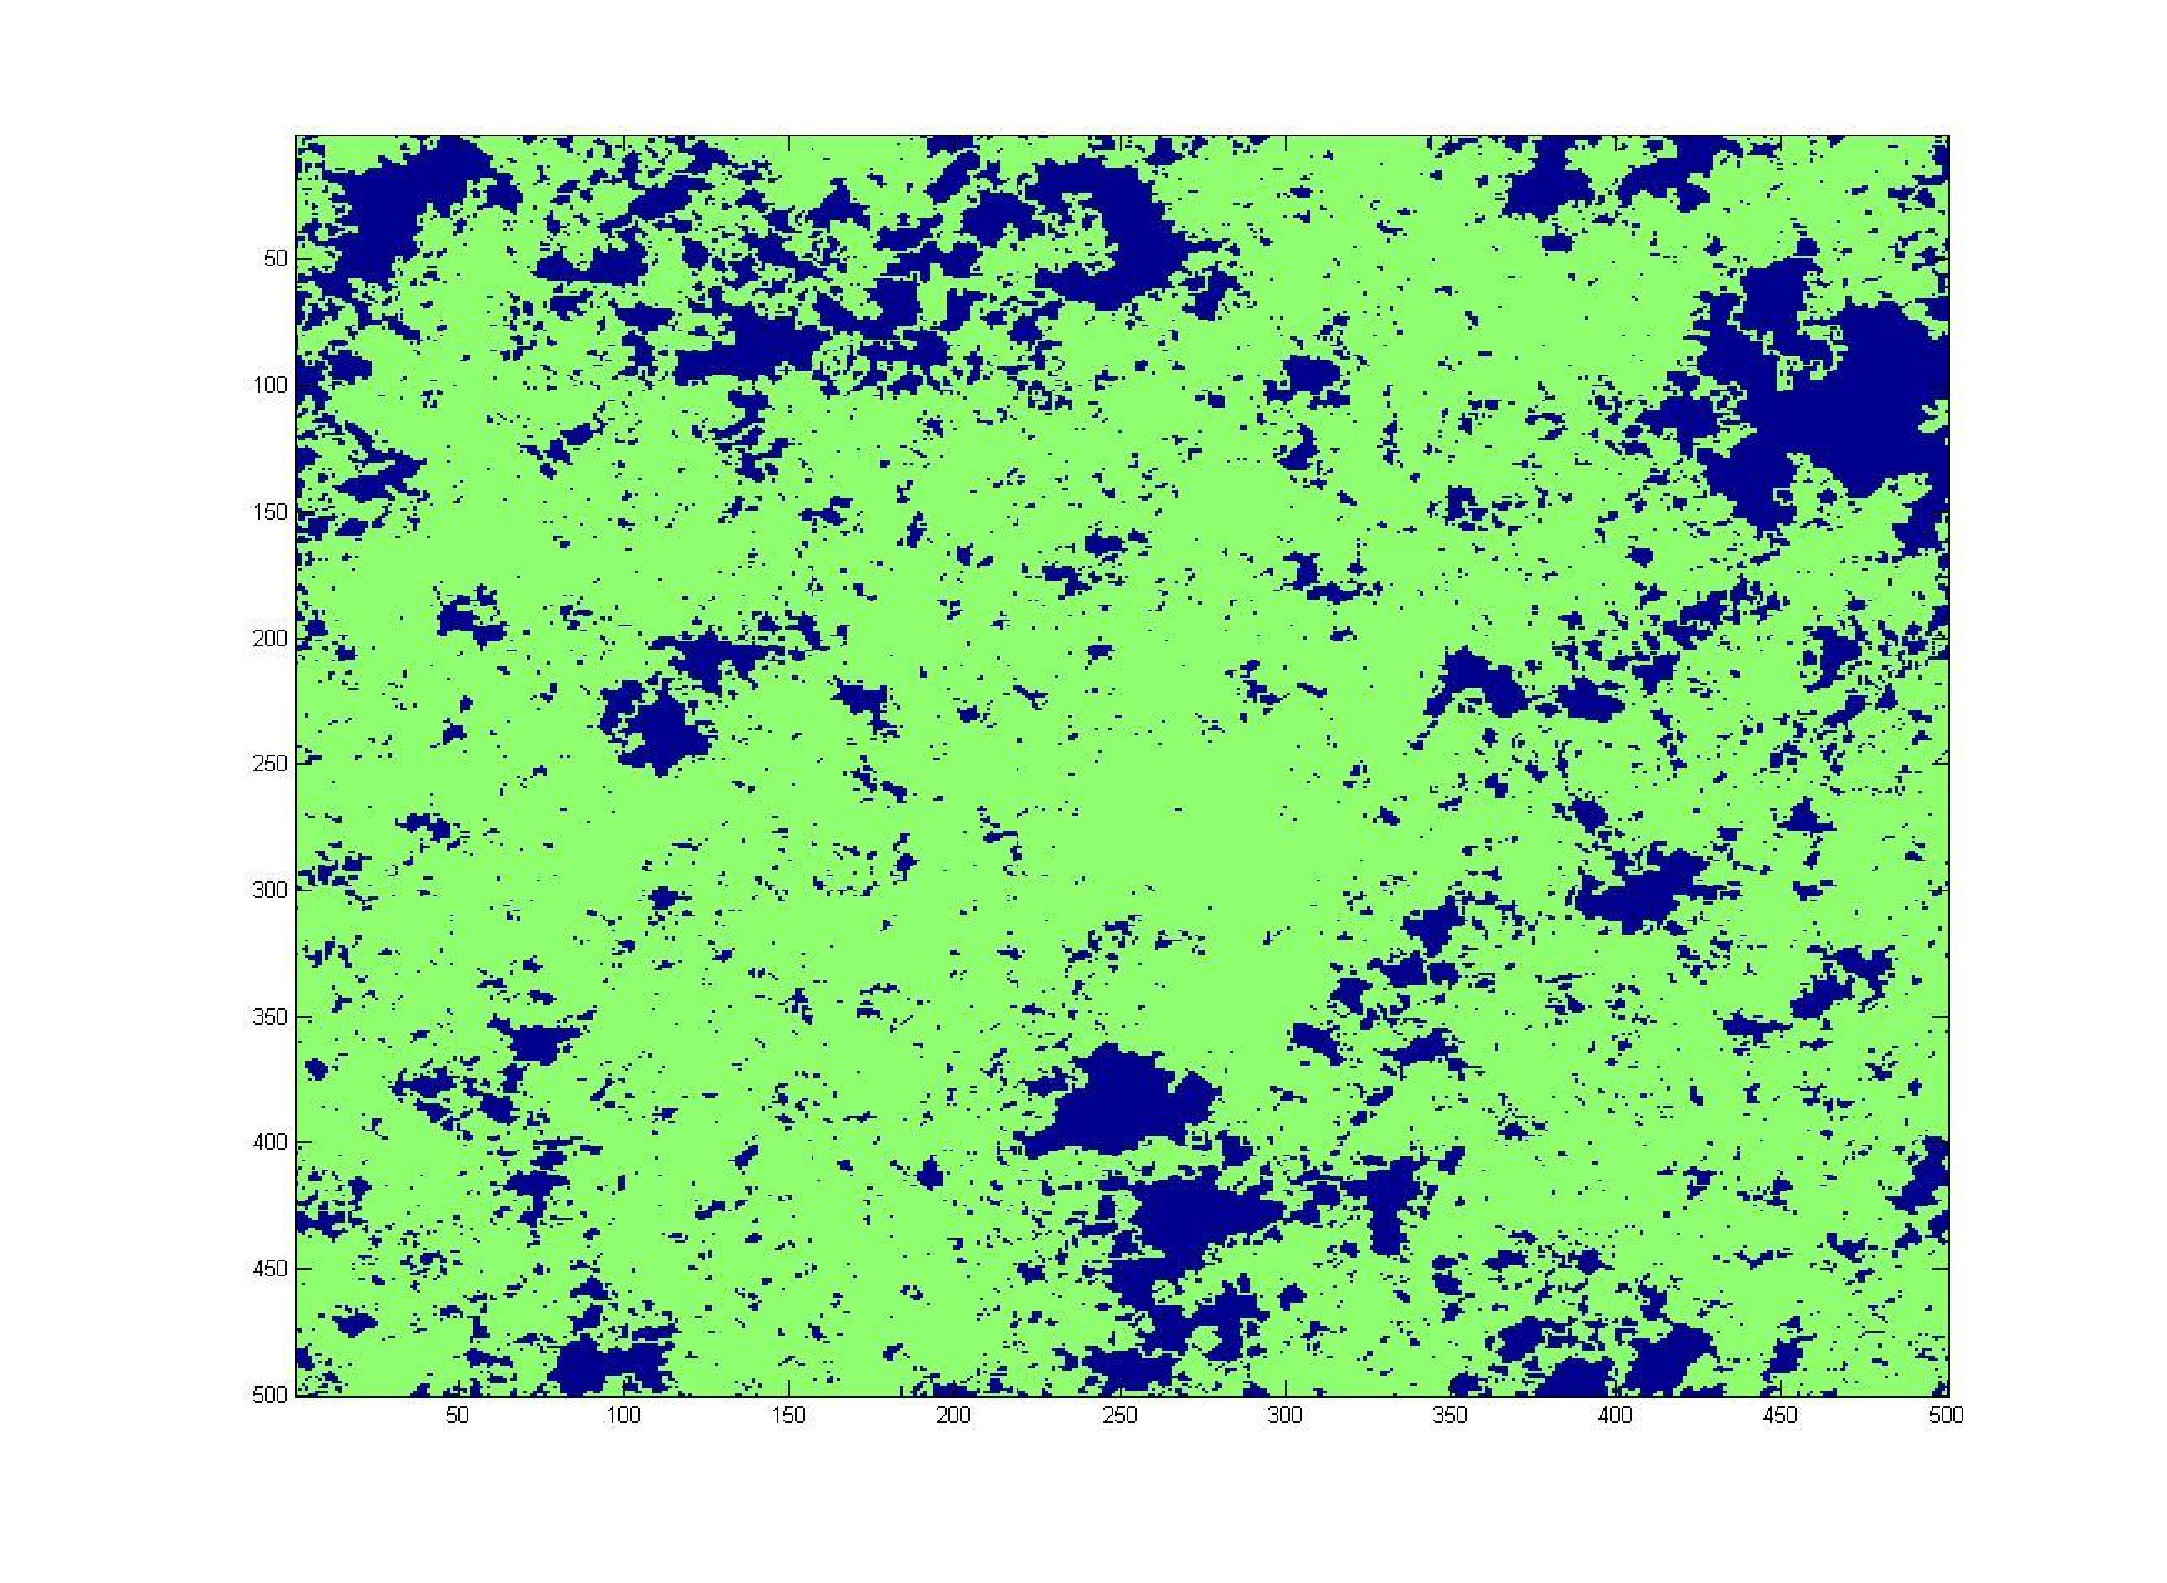
\includegraphics[height=70mm, width=100mm]{GRW_Torus_500_0.8.eps}
        \caption{GRW up to the time it visits 0.8 of the area of the torus}
        }
    \end{figure}

    \begin{figure}[htbp]
        \center{
        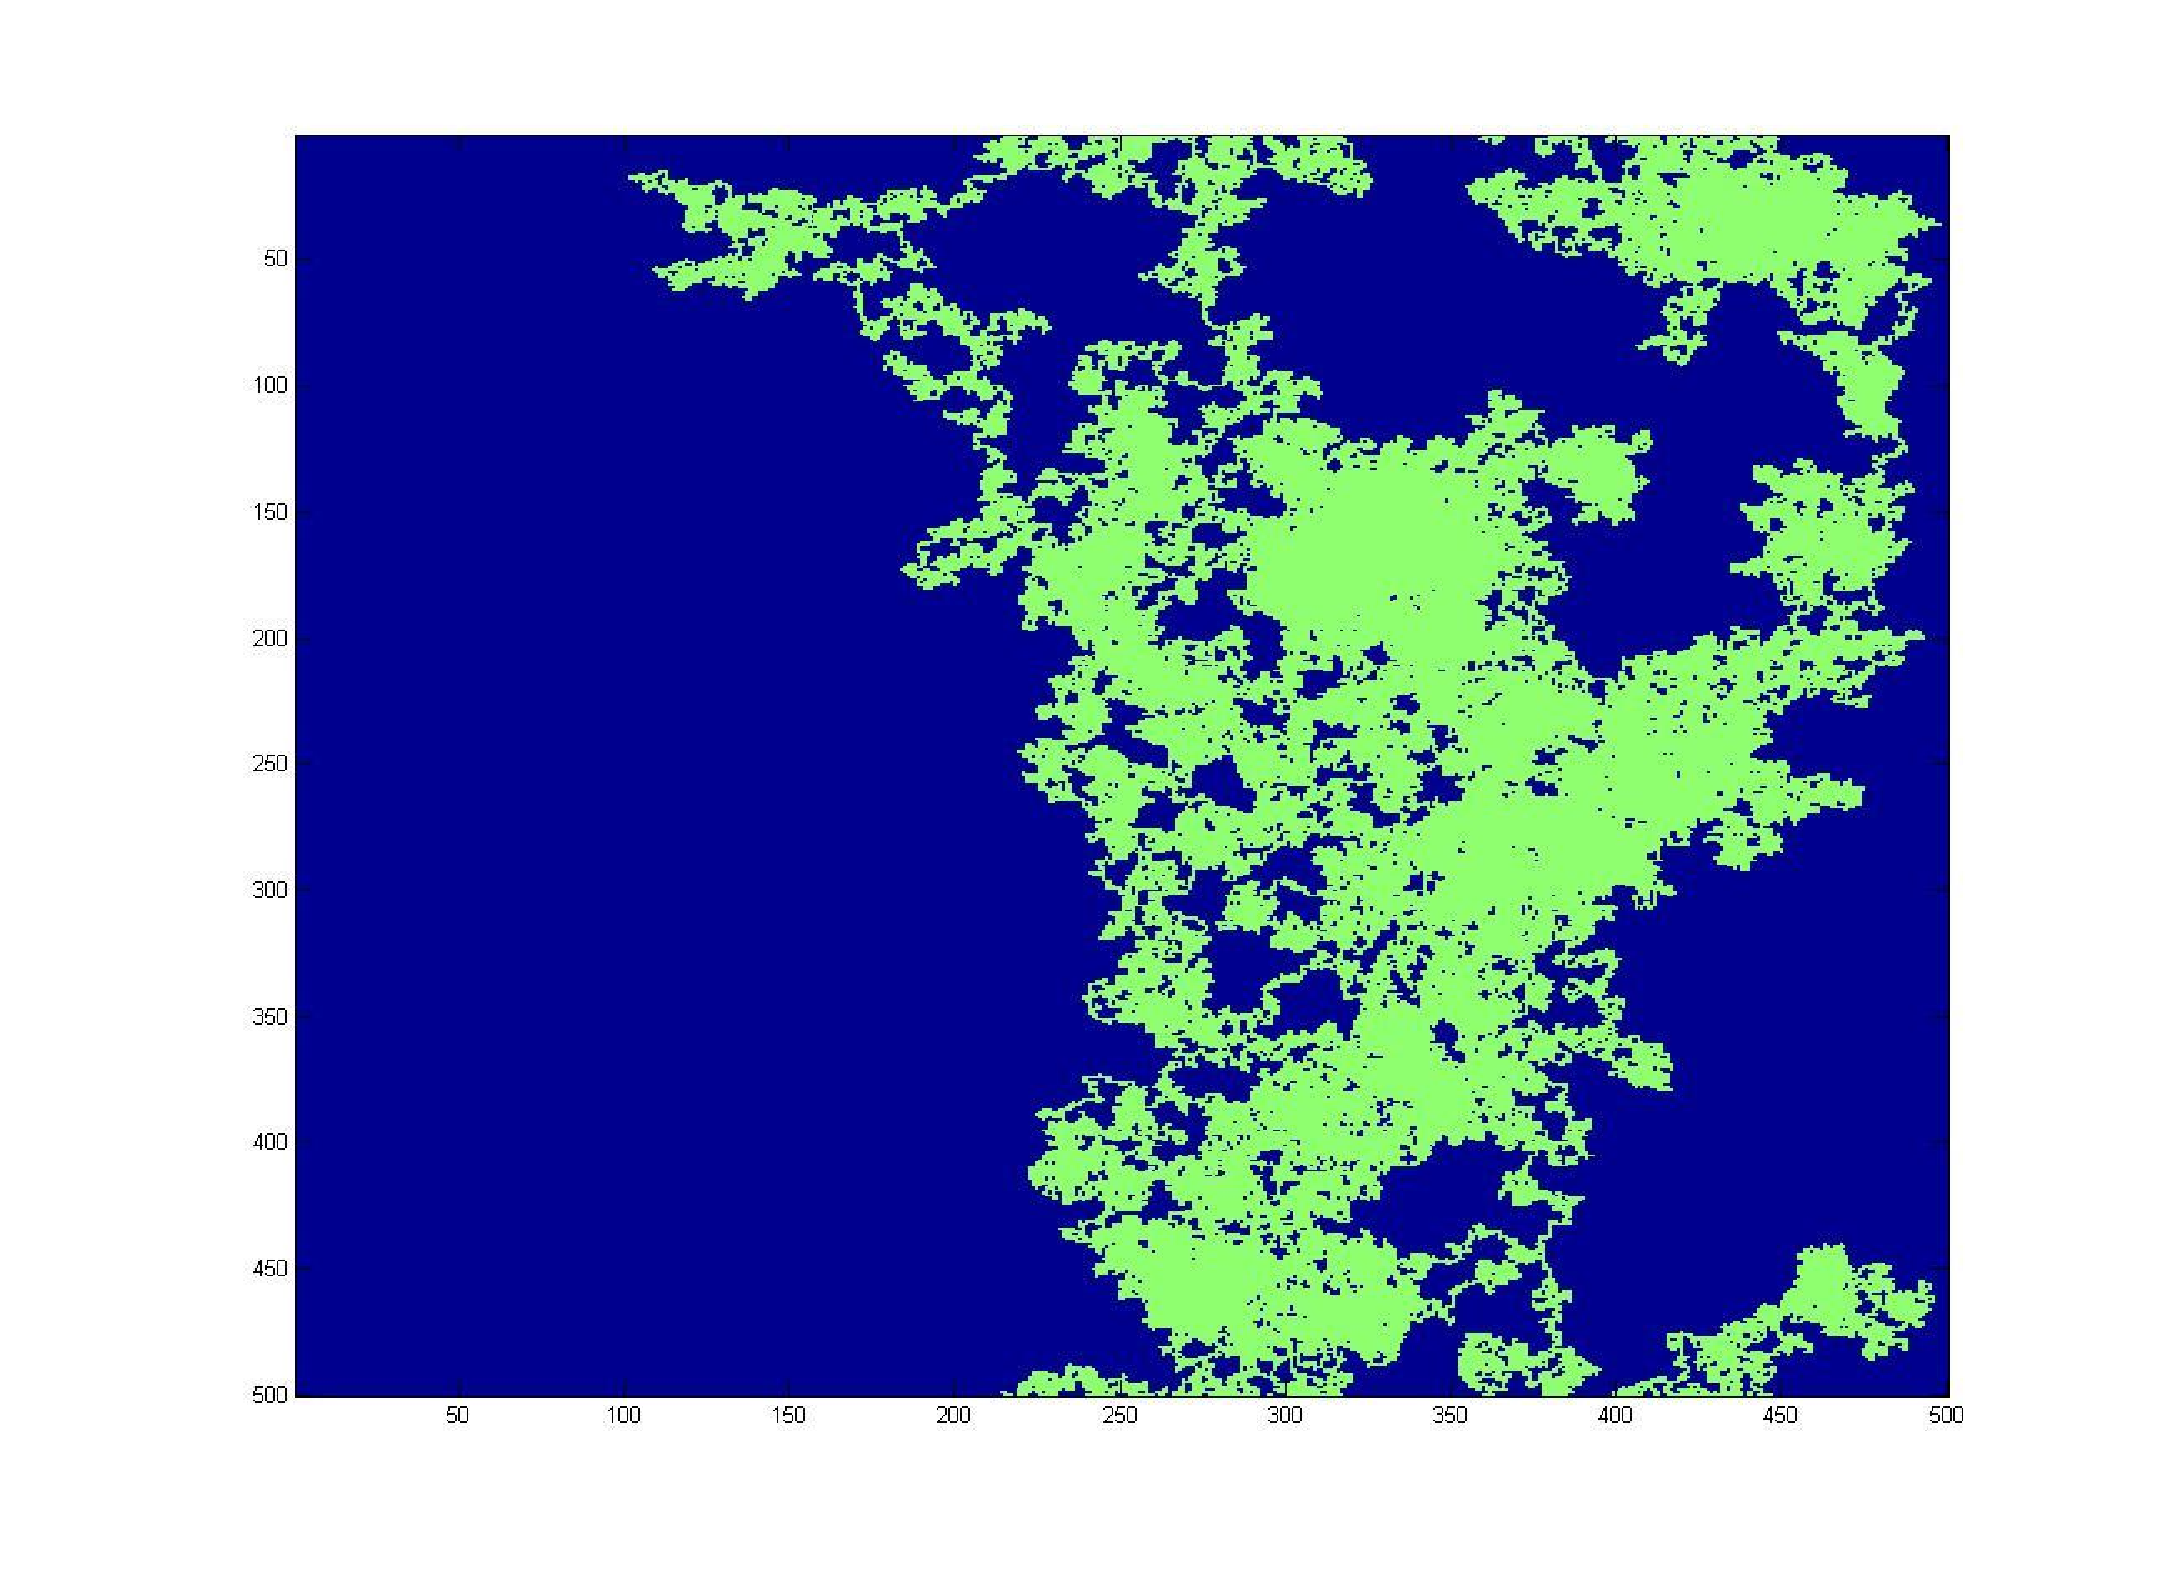
\includegraphics[height=70mm, width=100mm]{SRW_Torus_500_0.8.eps}
        \caption{SRW up to the time that \emph{GRW} visits at 0.8 of the area of the torus}
        }
    \end{figure}

  \begin{figure}[htbp]
        \center{
        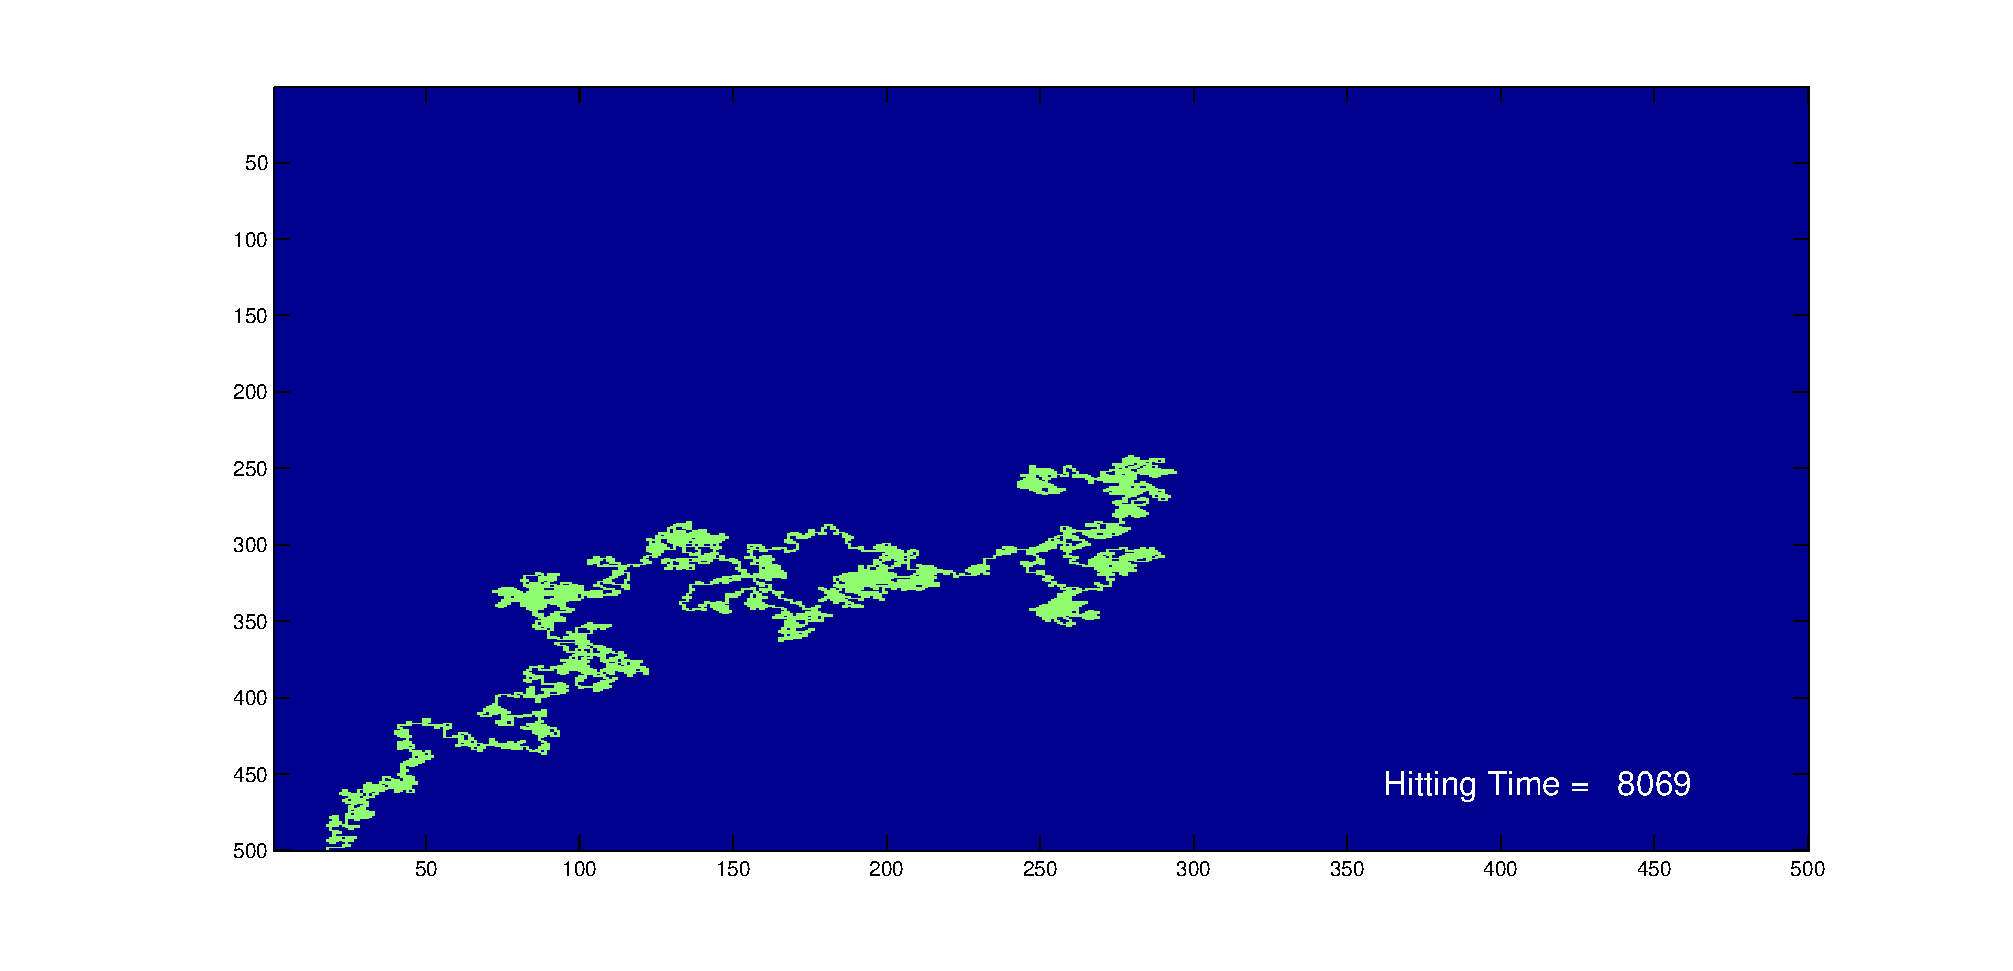
\includegraphics[height=70mm, width=100mm]{GRW_Box_500_BoundaryHittingTime.eps}
        \caption{GRW up to the first hitting time of the boundary of the box}
        }
    \end{figure}

    \begin{figure}[htbp]
        \center{
        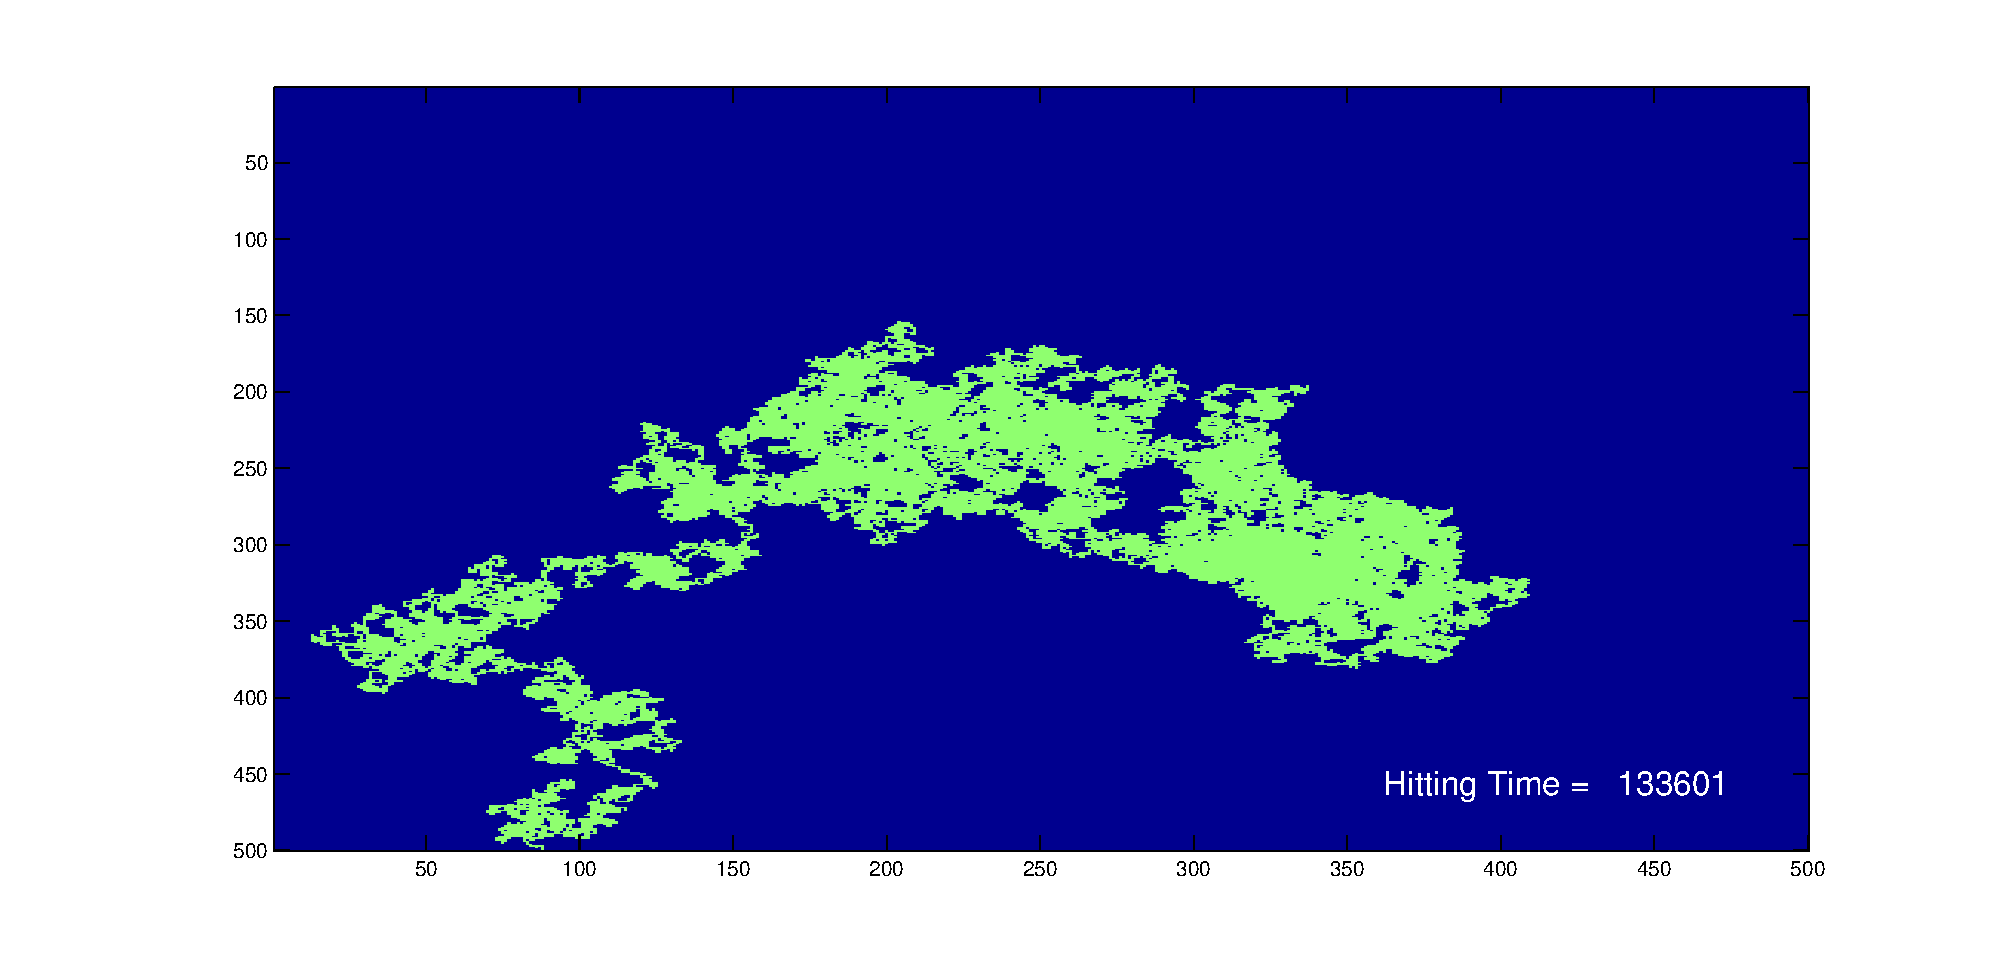
\includegraphics[height=70mm, width=100mm]{SRW_Box_500_BoundaryHittingTime.eps}
        \caption{SRW up to the first hitting time of the boundary of the box}
        }
    \end{figure}


%%%%%%%%%%%%%%%%%%%%%%%%%%%%%%%%%%%%%%%%%%%%%%%%%%%%%%%%%%%%%%%%%%%%%%%%%%%%%%%%%%%%%%%%%%
\section{Remarks and Open Questions}\label{sec:remarks}
%%%%%%%%%%%%%%%%%%%%%%%%%%%%%%%%%%%%%%%%%%%%%%%%%%%%%%%%%%%%%%%%%%%%%%%%%%%%%%%%%%%%%%%%%%

    One may consider a variant of the greedy random walk defined as follows.
    At each step from a vertex $v$, the random walk picks uniformly at random a non visited neighbor
    and moves to it. If all neighbors were visited, it picks one of them uniformly at random and moves to it.

    This walk may be beneficial to lower the expected \emph{vertex} cover time, for finite graphs of high degree.
    For example, it is obvious that in the clique $K_n$, the vertex cover time is $n$.

    For some graphs the expected edge cover time of this walk coincides with the one of GRW.
    For example, a similar treatment as the one of Section \ref{subsec:binary_tree}, yields that this is indeed the case for $d$-trees.

    \bigskip

    We conclude with a list several open questions.

    \enumlist{
    \item
        Show upper bounds on $T^E_G$ for other families of graphs.
        Interesting graph to look at could be a $d$-dimensional torus and a hypercube.

    \item
        It seems also interesting to analyze the GRW on graphs with power-law degree distribution. As on such graphs there are hubs
        of very large degrees and when visiting these the GRW will be very efficient.

    \item
        Show that the expected edge cover time of the GRW cannot be asymptotically larger than that of the SRW for any finite graph
        (This is true for graphs of even degree).
        Note that for $G = P_n$, a path of length $n$, when starting from the midpoint, the expected cover time of GRW
        and that of SRW or of the same order ($\Theta(n^2)$).

    \item
        Give bounds on the expected vertex cover time of the GRW for finite graphs.

    \item
        Define GRW mixing time and show that GRW mixing time is as fast as that of SRW (here \cite{ABLS06} is relevant, and also \cite{Madras2005} may be found useful).

    \item
        Give bounds on the expected hitting time of GRW for different graphs.


\bigskip
\noindent
The coming problems are regarding recurrence of GRW on infinite graphs.



    \item
        Show that the GRW on the ladder $\Z \times \Z_2$ is recurrent.

    \item
        Is GRW on $\Z^2$ recurrent? Is GRW diffusive on $\Z^d$, for all $d >1$?

    \item
        Prove that any graph rough isometric to the $\Z^3$ square lattice is transient. In particular any odd degree lattice.


    \item
        Show that if an infinite graph $G$ is nonamenable, then GRW on $G$ is transient.
 }

\section{Acknowledgements}
    We thank Itai Benjamini for proposing the model and for many valuable discussions,
    Shlomo Jozeph for suggesting the concatenation argument in Theorem \ref{thm:Z^d} and Gady Kozma for valuable comments on the first version of the paper.


\newcommand{\etalchar}[1]{$^{#1}$}
\begin{thebibliography}{ABLS06}

\bibitem[ABLS06]{ABLS06}
Noga Alon, Itai Benjamini, Eyal Lubetzky, and Sasha Sodin.
\newblock Non-backtracking random walks mix faster.
\newblock {\em Comm. Cont. Math.}, 9:585--603, 2006.

\bibitem[AKL{\etalchar{+}}79]{AKLLR79}
Romas Aleliunas, Richard~M. Karp, Richard~J. Lipton, L\'{a}szl\'{o} Lov\'{a}sz,
  and Charles Rackoff.
\newblock Random walks, universal traversal sequences, and the complexity of
  maze problems.
\newblock In {\em Proceedings of the 20th Annual Symposium on Foundations of
  Computer Science}, pages 218--223, Washington, DC, USA, 1979. IEEE Computer
  Society.

\bibitem[Ald91]{aldous1991random}
D.J. Aldous.
\newblock {Random walk covering of some special trees}.
\newblock {\em Journal of Mathematical Analysis and Applications},
  157(1):271--283, 1991.

\bibitem[AY]{AngelYaari}
Omer Angel and Yariv Yaari.
\newblock {Bridge burning walk on the complete graph and the $O(n)$ model}
\newblock {\em (private communication)}.

\bibitem[BGM10]{BGM}
Itai Benjamini, Ori~Gurel Gurel, and Ben Morris.
\newblock Linear cover time is exponentially unlikely.
\newblock 2010.
\newblock http://arxiv.org/abs/1011.3118.

\bibitem[BK89]{BroderKarlin89}
Andrei~Z. Broder and Anna~R. Karlin.
\newblock Bounds on the cover time.
\newblock {\em Journal of Theoretical Probability}, 2:101--120, 1989.

\bibitem[BW03]{BW03}
Itai Benjamini and David~B. Wilson.
\newblock Excited random walk.
\newblock {\em Elect. Comm. in Probab.}, 6:86--92, 2003.

\bibitem[Fei95]{Feige95lowerbound}
Uriel Feige.
\newblock A tight lower bound on the cover time for random walks on graphs.
\newblock {\em Random Struct. Algorithms}, 6:433--438, July 1995.

\bibitem[FS10]{FrSa10}
Tobias Friedrich and Thomas Sauerwald.
\newblock The cover time of deterministic random walks.
\newblock In {\em Proceedings of the 16th annual international conference on
  Computing and combinatorics}, COCOON'10, pages 130--139, Berlin, Heidelberg,
  2010. Springer-Verlag.

\bibitem[MW05]{Madras2005}
Neal Madras and C.~Chris Wu.
\newblock Self-avoiding walks on hyperbolic graphs.
\newblock {\em Comb. Probab. Comput.}, 14:523--548, July 2005.

\bibitem[Pem07]{Pem07}
Robin Pemantle.
\newblock A survey of random processes with reinforcement.
\newblock {\em Probability surveys}, 4:1--79, 2007.

\end{thebibliography}

\end{document}
